%TC:envir minttcb [ignore] xall

\chapter{VTOL-AirSim User Guide}\label{chp:userguide}

This chapter will be a detailed guide involving the setup, configuration, and basic uses of Microsoft AirSim and our extension to AirSim, VTOL-AirSim. Sections~\ref{sec:description_airsim}--\ref{sec:basic_use_airsim} are written for those who have never used AirSim previously, and serves as an introduction to AirSim. Sections~\ref{sec:vtolairsim}--\ref{sec:vtol_examples} are about VTOL-AirSim and examples of how to use it.

All instructions throughout this text are written for Linux users. The instructions have been tested on Arch Linux and Ubuntu 20.04 --- the latest Long Term Support (LTS) release as of this writing --- and are written with a focus on Ubuntu users.

If this is your first time using AirSim, regardless of your use case, it is recommended that you follow the setup guide described in this chapter before continuing to the advanced chapters. This will help you to be aware of the various components involved in a complete simulation environment, which will be very beneficial knowledge when debugging a problem or attempting to add functionality to the sim later.

\section{Description of AirSim}\label{sec:description_airsim}

It is important to first understand what exactly AirSim is before setting it up. AirSim should be thought of not as a single, self-contained simulator program, but rather as a collection of simulation tools which you can link together in various ways and interface with at various levels. Because of this, there are multiple ways to use AirSim, and individual AirSim-based simulations can appear to be quite different from one another depending on which components are used. Nevertheless, there are two parts to any complete AirSim simulation: an environment (the server) and one or more clients interacting with the environment. While it is technically possible to have zero clients connected to the environment server, the result would be an environment containing one or more vehicles that never perform any actions, and this is not very useful. Thus, any complete AirSim simulation has at least one connected client. What follows is a brief description of these two parts and their major components.

Note that for simplicity, the following sections are worded in terms of a single vehicle in the simulation; however, AirSim has full multi-vehicle support, so any mention of a single vehicle can be substituted with multiple vehicles. In addition, AirSim also has a car mode, but it is outside the scope of this work.

\subsection{Definitions}\label{sec:definitions}
The following terms can have different meanings depending on the context, and so we have decided on some fixed definitions for this text.

\begin{itemize}
    \item \textbf{mesh} --- The collection of vertices, edges, and faces that make up the graphical representation of an object.
    \item \textbf{model} --- The dynamic model of the vehicle; or, in other words, the equations of motion, control inputs and motor outputs that are particular to a vehicle or vehicle type.
    \item \textbf{viewport} --- The area of the screen in which rendered graphics are displayed to the user.
\end{itemize}


\subsubsection{Environment}
The environment is a 3D graphics application which has been compiled for use with AirSim. The environment contains a scene made up of various meshes, which may be static or mobile. The vehicle is an animated mesh representing the state of the aircraft which the user controls. The graphics engine rendering the environment and the vehicle is \textit{Unreal Engine}: a game engine used for producing high-end graphics video games, but which can also be a useful tool for engineering simulations. When the environment is running, Unreal Engine is responsible for the following tasks: render images for the simulated camera sensor from the environment; handle vehicle collisions with objects in the scene; animate any moving parts of the vehicle plus the movement of the vehicle itself; and display rendered images to the user's viewport. Meanwhile, invisible to the user, AirSim performs a number of other tasks, namely: simulate the physics of the vehicle and the non-camera sensors; process control inputs and simulate motor responses --- either through its own autopilot stack for multirotors, SimpleFlight, or by interfacing with an external autopilot such as PX4 --- communicate with Unreal Engine about the vehicle's state and the physics of any collisions that occur; and run a remote procedural call (RPC) server, which processes commands sent by the client.

\subsubsection{Client}
The client is a process initiated by the user which sends commands to the server (the RPC server which runs inside the environment). Any client is initiated independently from the environment. There can be multiple clients running and simultaneously passing data to and from the server. Clients can be created, shut down, or restarted any number of times while the server is running. The environment is initiated first, because it is the server, and any clients are initiated after. This is because a client won't perform any actions until a connection with the server is established, and if it tries to create a connection but can't, it will close with an error.

\subsection{Outline of AirSim Components}
We have just explained the two primary parts of an AirSim simulation: the environment and a client. With that knowledge in hand, we will now outline the major components of AirSim.

\begin{itemize}
    \item AirLib --- The core \CC code of AirSim consisting of many subcomponents, including:
    \begin{itemize}
        \item physics (dynamics, drag model, thrust and torques, collision handling)
        \item non-camera sensor models
        \item control inputs and motor responses
        \item a small, self-contained multirotor autopilot called SimpleFlight
        \item interfaces for the autopilots PX4 and Ardupilot
        \item RPC server and client
    \end{itemize}
    \item MavLinkCom --- \CC library that uses MavLink to communicate with PX4 or Ardupilot
    \item Python client --- a Python wrapper around the \CC RPC client found in AirLib
    \item Compiled environments (binaries) --- a selection of prebuilt, downloadable environments
    \item Unreal Engine plugin, plus a simple example project named Blocks
    \item Unity plugin --- a plugin for the Unity game engine, which will not be covered in this text
\end{itemize}

Each of these components may or may not be used in a given AirSim simulation, but they are all part of the stack of software that AirSim offers. It is up to the user to decide which of these components to use, interface with, or modify based on the needs of the project at hand.

\section{Basic Setup: Prebuilt Environment}\label{sec:basic_setup}

We will now begin with the most basic setup of AirSim: using a prebuilt environment. This is the least configurable way to use AirSim, but it is the fastest and easiest way to get an AirSim simulation running on your machine. Prebuilt environments allow for some configuration by way of a settings file. For some projects, the settings offered for prebuilt environments may be sufficient.

The first step is to download a prebuilt environment from the AirSim GitHub repository. The repository is located online at \url{https://github.com/microsoft/AirSim}. This is the repository containing all of the source code behind the various components outlined in the previous section. On the right of the page you will see several sections containing information about the repository. The first section is labeled \textbf{About}, and underneath it is a section labeled \textbf{Releases}. Click on the header \textbf{Releases} to go to the AirSim Releases page. Alternatively, you can go directly to the page at \url{https://github.com/microsoft/AirSim/releases}.

\subsection{Explanation of GitHub Releases}
If you are not familiar with the concept of releases, it is essentially a snapshot of the software contained in the repository at a certain moment (i.e., at a specific commit). Developers create releases at particular commits that they have deemed important enough in some way to warrant packaging the code in a deliverable format, and to give the commit a special label called a \textit{tag}. A commit can be tagged without creating a release (hence the \textbf{Tags} subsection on the Releases page), but a release is always associated with a tag. Releases are most often used to mark a version of the software. Every release on GitHub includes links to download a copy of the source code at that particular commit, but they may also include release notes or additional files for others to use. Often, the managers of a repository will include links to binary files which have been compiled from the source code at that release. This is how the AirSim developers structure their releases.

\subsection{Download an Environment}
On the AirSim Releases page, you will find links to download environments built by the AirSim team. AirSim usually creates two releases for every new version: one containing environments compiled for Windows, and another with environments compiled for Linux; the source code is the same in each. Scroll down the page until you find the most recent release for Linux. The release should be titled in the form of \texttt{vX.Y.Z --- Linux}, where X, Y, and Z are numbers making up the version of that release. For example, as of this writing, the most recent release is titled \texttt{v1.5.0 --- Linux}; it contains environments built for Linux using version 1.5.0 of the AirSim source code. Be sure that you find the release for Linux and not Windows --- although the files may have the same names, the environments listed under the Windows release are \textit{not} compatible with Linux.

Once you have found a Linux release, at the bottom of the release notes you will find all the files that are a part of the release under the expandable section labeled \textbf{Assets}. Expand this section by clicking on the label, after which you should see a number of links pertaining to each environment that has been built for Linux. (For brief descriptions of the available environments, see Appendix~\ref{apdx:list_of_envs}.) A good environment to start with is the AirSimNH environment (\textit{NH} meaning \textit{Neighborhood}). Download the ZIP file for this environment and unzip it to a directory of your choice.

Finishing this step will give you the first part of AirSim: the environment. You still need to be able to start a client before you can do anything with AirSim. To start a client, we will use AirSim's Python interface with one of the example Python scripts that AirSim provides.

\subsection{Create a Python Virtual Environment for AirSim}\label{sec:virtual_env}
If you haven't used a Python virtual environment before, it is very easy to create and use one. What it does is create an isolated space (a directory) where non-built-in Python packages will be installed to and searched for when importing or executing code from those packages. All you have to do is create the virtual environment and \textit{activate} it each time you want to use it; you then \textit{deactivate} it when you don't.

It is strongly recommended that you create an entirely fresh Python virtual environment specifically for AirSim. As of this writing, the \ci{airsim} Python package has a dependency on a deprecated and very old package named \ci{msgpack-rpc-python}, which itself has other outdated dependencies that can create problems if you integrate it with your other Python virtual environments, or your user-wide or system-wide Python environments.

You can place the virtual environment wherever you like. It is common to create a folder dedicated to storing virtual environments, often in the user's home directory. The following instructions will create a directory named \ci{.virtualenvs} in the home directory; feel free to replace the path with whichever path and directory name you choose.

First, create a directory to store virtual environments. If you already have a directory that fulfills this purpose, skip this step.
\begin{minttcb}{bash}
    mkdir ~/.virtualenvs
    cd ~/.virtualenvs
\end{minttcb}
\noindent Next, create a virtual environment. We will name it \ci{airsim}.
\begin{minttcb}{bash}
    python3 -m venv airsim
\end{minttcb}
This will create a folder at the current working directory named \ci{airsim} containing a brand new virtual environment. Note that a virtual environment can only contain a single version of Python, and the above command will create a virtual environment according to whichever Python version the \ci{python3} command points to on your system. If you need to some other Python version, replace the number 3 with the specific version you need. For example, if you need to use Python 3.9 but \ci{python3} points to Python 3.8 (verify with the command \ci{python3 --version}), replace \ci{python3} in the above command with \ci{python3.9}. \textit{Warning: be sure you are using Python 3. Do not attempt to use Python 2 with AirSim}.

To activate the new virtual environment, you need to source its \ci{activate} script, which can be done with the following command.
\begin{minttcb}{bash}
    source ~/.virtualenvs/airsim/bin/activate
\end{minttcb}
This will do a number of things to configure your shell's environment to use the \ci{airsim} directory for importing and installing new Python packages. You have now \textit{activated} your virtual environment for AirSim. Whenever you need to use your AirSim virtual environment in the future, you must either run the above command directly, or, to make it easier to remember, you can create an alias for that command and then use the alias. To stop using the virtual environment, run the command \ci{deactivate} in the terminal.

If you would like a setup that is a bit more convenient and robust for activating and deactivating virtual environments, see Appendix~\ref{apdx:adv_setup_python_venv}.

\subsubsection{Install the AirSim Python Package}
The AirSim Python package can be installed through \ci{pip}. Activate your virtual environment, ensure that \ci{pip} is up-to-date, then install the \ci{airsim} package.
\begin{minttcb}{bash}
    source ~/.virtualenvs/airsim/bin/activate
    pip install --upgrade pip
    pip install airsim
\end{minttcb}

\subsubsection{Get the Python Client Example Scripts}
The easiest way to get all the example scripts for using the Python client from AirSim is by cloning the AirSim GitHub repository. Assuming you have added an SSH key for your machine to your GitHub account (see Appendix~\ref{apdx:github_config}), you can run the following command in a terminal to clone the repository using SSH.
\begin{minttcb}{bash}
    git clone git@github.com:microsoft/AirSim
\end{minttcb}

\section{Basic Use}\label{sec:basic_use_airsim}

This section explains the most basic method of using AirSim.

\subsection{Run the Neighborhood Environment}
Open a terminal and navigate to where you placed the \ci{AirSimNH} folder that was extracted from the \ci{AirSimNH.zip} archive, then go to \ci{AirSimNH/LinuxNoEditor}. This \ci{LinuxNoEditor} folder is created by Unreal Engine; it follows a naming convention which indicates that it is a packaged, standalone application built for Linux that doesn't require the Unreal Editor to run.

\begin{figure}[ht]
    \centering
    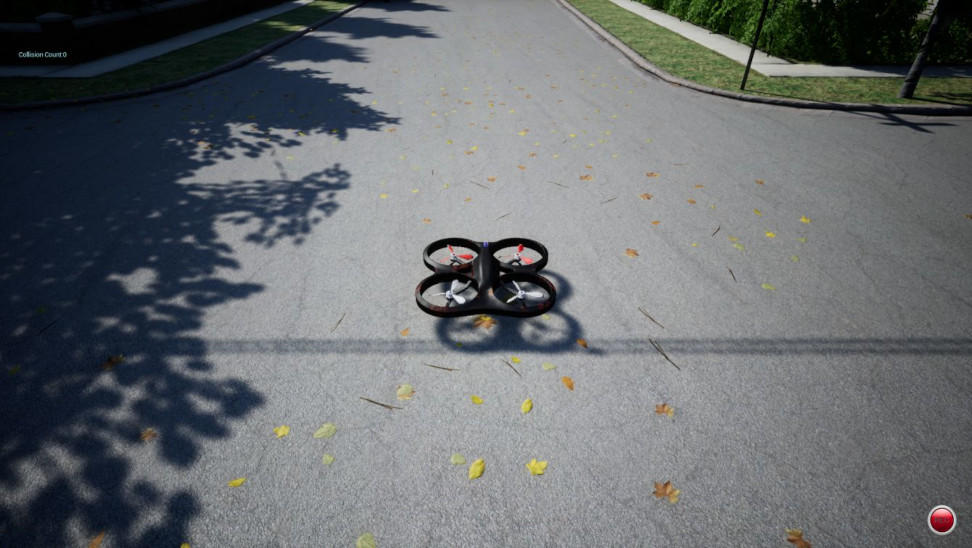
\includegraphics[height=250pt]{figures/airsimnh}
    \caption[AirSim Neighborhood Environment]{
        AirSim running in the Neighborhood environment.}%
    \label{fig:airsimnh}
\end{figure}

To start the environment, run the script \ci{AirSimNH.sh} found inside this directory. The script simply sets the application (i.e., the compiled binary) file named \ci{AirSimNH} located under \ci{AirSimNH/Binaries/Linux} to be executable, then executes it. This will start the application, and you will see a new blank window open. A dialog box will appear asking if you would like to use the car simulation. Click \textbf{No} to proceed. The window will then begin rendering the Neighborhood environment with a lone quadrotor (Fig.~\ref{fig:airsimnh}). You are now running the AirSim server. However, because there are no clients running, the quadrotor will remain stationary until a client connects and sends commands to it.

\subsection{Start the Client}
It's time to start an AirSim client. We will use one of the example scripts for using the Python client contained in the AirSim repository. Create a new terminal session and activate your AirSim virtual environment. Navigate to the directory where you cloned the AirSim repository and find the Python script \ci{AirSim/PythonClient/multirotor/takeoff.py}, then run the script. The commands for these steps are as follows:
\begin{minttcb}{bash}
    source ~/.virtualenvs/airsim/bin/activate
    cd <path to AirSim repository>/PythonClient/multirotor
    python takeoff.py
\end{minttcb}
In the AirSim window, you should see the multirotor take off, reach a certain height, then descend and land back on the pavement. Congratulations, you have just executed a complete AirSim simulation. In the next sections, we will shift our focus to VTOL-AirSim.

\section{VTOL-AirSim}\label{sec:vtolairsim}
Our additions to AirSim for simulating eVTOL aircraft is called \textit{VTOL-AirSim}. The previous sections in this chapter apply equally well to VTOL-AirSim, as it is simply AirSim with extended capabilities. From a user standpoint, the biggest difference is the addition of a new \textit{simulation mode}. AirSim's three simulation modes are: \ci{Multirotor}, \ci{Car}, and \ci{ComputerVision}. In each mode, a multirotor, or a car, or a controllable camera will spawn, respectively, and each type has its own set of control schemes. The simulation mode is specified in the settings file (Section~\ref{sec:settings_file}); or, if it isn't specified there, AirSim displays the dialog box when you start an environment asking if you would like to use the car simulation, after which it will start the \ci{Car} or the \ci{Multirotor} mode according to the user's selection. In VTOL-AirSim, we added a fourth simulation mode: \ci{Vtol}. In this mode, a tiltrotor vehicle will spawn, and it has its own set of control schemes, which we cover in the examples given in Section~\ref{sec:vtol_examples}.

\subsection{The Tiltrotor Model}\label{sec:tiltrotor_model}
It is important to know that the dynamic model for the tiltrotor vehicle is the E-flite Convergence aircraft (Fig.~\ref{fig:convergence}). This is because another project by the MAGICC Lab, named VTOLsim, had previously created a dynamics simulation utilizing a model of the Convergence aircraft. Given that we already had the various physical and aerodynamic parameters of the model, we had the actual hardware, and the Convergence was one of the airframes supported by the PX4 Autopilot, we chose to use it for the first iteration of an eVTOL vehicle in AirSim.

\begin{figure}[ht]
    \centering
    \begin{subfigure}[b]{0.42\textwidth}
        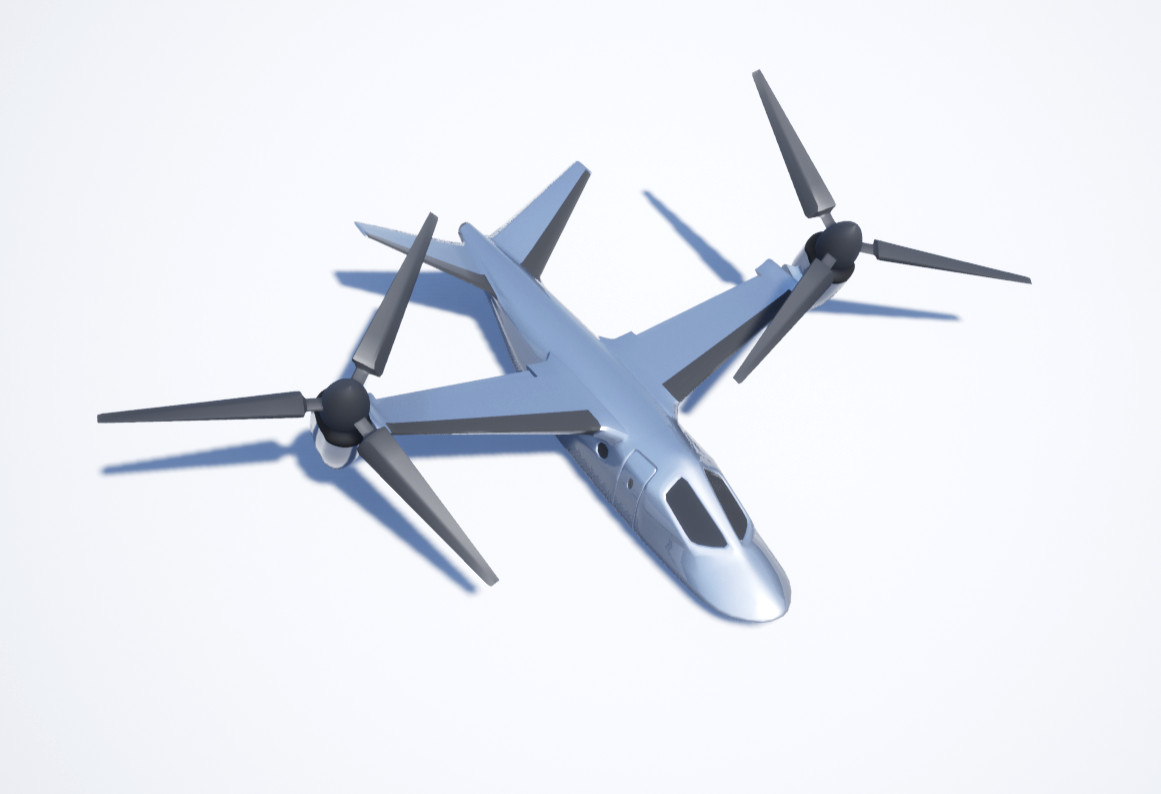
\includegraphics[width=\textwidth]{figures/tiltrotor_solo3}
        \caption[Tiltrotor vehicle used in VTOL-AirSim]{
            The tiltrotor vehicle in VTOL-AirSim.}%
        \label{fig:tiltrotor_solo}
    \end{subfigure}
    \qquad
    \begin{subfigure}[b]{0.42\textwidth}
        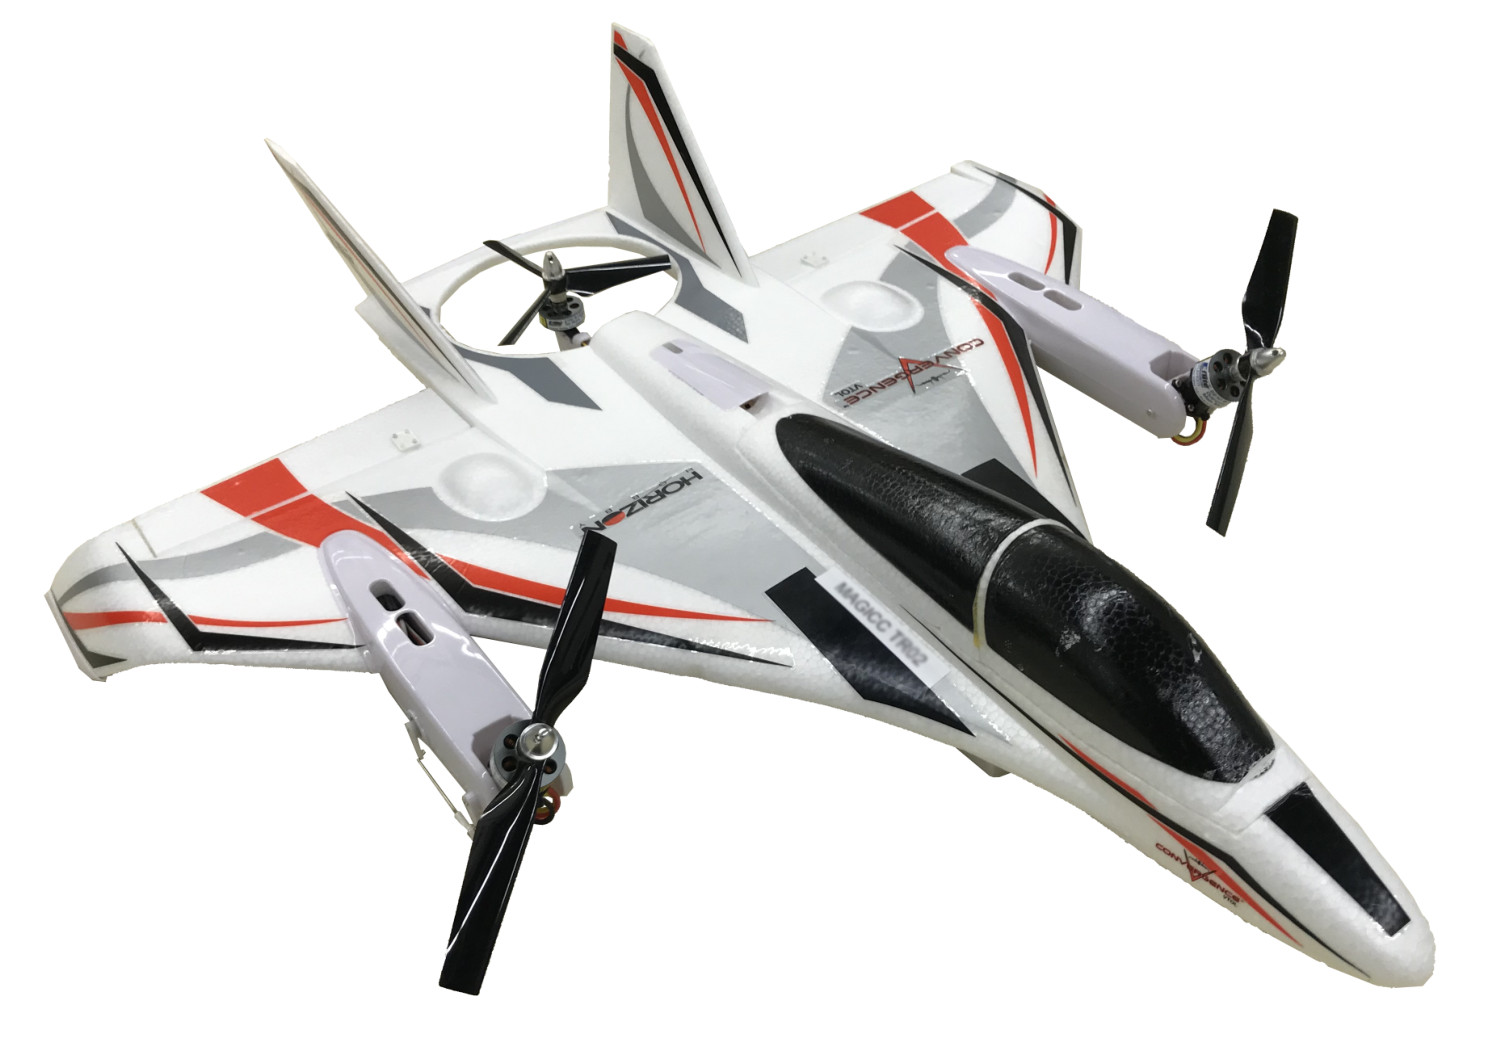
\includegraphics[width=\textwidth]{figures/convergence}
        \caption[E-flite Convergence aircraft]{
            The E-flite Convergence aircraft that serves as the dynamic model.}%
        \label{fig:convergence}
    \end{subfigure}
    \caption[Tiltrotor vehicle in VTOL-AirSim compared with E-flite Convergence]{
        Comparison of the tiltrotor mesh in VTOL-AirSim and the E-flite Convergence.}%
    \label{fig:tiltrotor_convergence}
\end{figure}

Note that the Convergence actually has three rotors --- it is a \textit{tri-tiltrotor} design --- but the tiltrotor in VTOL-AirSim only has two. We were not able to find a suitable mesh for a tri-tiltrotor aircraft when we created the tiltrotor vehicle. In addition, the Convergence is a small UAV that requires a rear rotor for stability, while a passenger-size tiltrotor would typically not have a rear rotor, so we decided that this was acceptable. However, internal to VTOL-AirSim, the tiltrotor does in fact have a rear rotor; it is simply not a part of the visual representation.


\subsection{Environments Available in VTOL-AirSim}
One component of AirSim that is not shared by VTOL-AirSim is the availability of AirSim's prebuilt environments. Because we do not have access to the Unreal Engine assets that the AirSim developers used to create their environments (other than the Blocks environment), VTOL-AirSim can't be compiled into, say, the Neighborhood environment. There are, however, two environments which we have compiled for VTOL-AirSim: Blocks, and CityBlocks. More information on the CityBlocks environment is in Section~\ref{sec:download_cityblocks}, and this is the environment we use in the VTOL-AirSim examples.

\section{The Settings File}\label{sec:settings_file}

There are many settings available for configuring the AirSim environment. All settings for AirSim are placed in a \ci{settings.json} file at the path \ci{~/Documents/settings.json}. For the official documentation on most of the available settings, go to \url{https://microsoft.github.io/AirSim/settings}. This section will outline the most important configuration options for VTOL-AirSim pertaining to eVTOL aircraft.

\subsection{Settings Are Read at Runtime}
At startup, AirSim checks for a JSON file at \ci{~/Documents/settings.json}, then, if it exists, it reads the file's contents and attempts to apply all the settings that are recognized. The settings file is read at the time of initialization; in other words, it is performed at runtime. This means that if a value for any setting is invalid, the application will generally crash during startup. In addition, the file must strictly follow official JSON syntax; if there are any syntax errors, the JSON parsing library that AirSim uses will throw an exception of type \ci[cpp]{std::invalid_argument}, causing the application to crash without printing any helpful information as to why it crashed. Be aware of this when you edit the settings file, and know that this is a common cause of startup crashes.

A key-value entry (i.e., a setting and a chosen value for that setting, which are written in the format \ci[text]{"key": "value"}) is valid if the AirSim environment was compiled with support for it. For example, the entry \ci[text]{"SimMode": "Vtol"} is valid only if using an environment that was compiled with VTOL-AirSim. If you specify that same entry and then run one of AirSim's prebuilt environments, the application will crash at startup because AirSim does not include \ci[text]{"Vtol"} as a possible simulation mode in its source code.

\subsection{Settings for VTOL-AirSim}
With the addition of the new \verb|Vtol| simulation mode, several new configuration options were added. The affected settings are outlined in the following list.

\begin{itemize}
    \item \ci{SimMode}
    \begin{itemize}
        \item Added new possible value: \ci{Vtol} (case insensitive)
        \item Explanation: Set the value to \ci{Vtol} to fly an eVTOL aircraft (currently tiltrotor only).
    \end{itemize}
    \item \ci{Vehicles}\ldots\ci{VehicleType}
    \begin{itemize}
        \item Added two new possible values: \ci{VtolSimple}, \ci{PX4Vtol} (case insensitive)
        \item Explanation: The default is \ci{VtolSimple}, which runs dummy firmware that simply passes through any PWM commands sent to it. Set this to \ci{PX4Vtol} to run VTOL-AirSim with PX4, as in the example in Section~\ref{sec:vtol_px4}.
    \end{itemize}
\end{itemize}

\section{How to Fly eVTOL Aircraft --- Examples}\label{sec:vtol_examples}
In this section we walk you through several complete examples of flying eVTOL aircraft in VTOL-AirSim. In the first example (Section~\ref{sec:vtol_geometric_control}), we cover a full demonstration that includes trajectory generation and following by sending PWM commands to AirSim. In the second example (Section~\ref{sec:vtol_teleport}), rather than sending control inputs to AirSim, we show how to override the vehicle's state in AirSim --- also referred to as \textit{teleporting} the vehicle --- for the case of utilizing an external dynamics simulation. In the third example (Section~\ref{sec:vtol_px4}), we show how to integrate the PX4 Autopilot in which we create and send a mission for the PX4 flight controller to execute and fly the aircraft.

As with the other simulation modes in AirSim, VTOL-AirSim comes with one mesh for the \verb|Vtol| vehicle in the form of a simple tiltrotor. Therefore, this is the aircraft that we use in each of the examples. We will also use the CityBlocks environment in these examples, which is one of two environments that we provide (the other being the Blocks world). If you are interested in changing what is available in VTOL-AirSim see Chapter~\ref{chp:extending} for information on how to get started.

\subsection{Required Settings}
For the first two examples in this section, \textit{Geometric Controller With PWM Commands} (Section~\ref{sec:vtol_geometric_control}) and \textit{Teleporting} (Section~\ref{sec:vtol_teleport}), you should have the following settings in your \ci{settings.json} file. As always, it should located at \ci{~/Documents/AirSim}.
\begin{minttcb}[title={Required Settings for eVTOL Examples}]{json}
{
  "SettingsVersion": 1.2,
  "SimMode": "Vtol",
  "ClockSpeed": 1.0,
  "LogMessagesVisible": false,
  "Vehicles": {
    "uav0": {
      "VehicleType": "VtolSimple"
    }
  }
}
\end{minttcb}

You can lower the \ci{ClockSpeed} setting if it appears that your machine is struggling to run the simulation. Also, the setting \ci{"LogMessagesVisible": false} is optional; however, when recording video or screenshots for presentations, it's usually best to disable the log messages that are displayed in the window.

\subsection{Download the CityBlocks Environment}\label{sec:download_cityblocks}
The CityBlocks environment is an environment that we created for use with VTOL-AirSim that is filled with static buildings, skyscrapers, streets, fields, and water. It was purchased and downloaded from the Unreal Engine Marketplace and afterwards modified to mimic the Blocks environment file structure; hence, we gave it the name \textit{CityBlocks}.

The compiled CityBlocks environment is available on the MAGICC Lab's Box storage at \url{https://byu.box.com/v/magicc-airsim-cityblocks}. Download the ZIP file and extract the archive to somewhere on your machine. You can then run the CityBlocks application by executing the script \ci{LinuxNoEditor/CityBlocks.sh}, just as you would for the official environments provided by AirSim. In the following examples, the instruction ``run the CityBlocks environment'' means to execute this script.

\subsection{Setup for the Python Client for VTOL-AirSim}
To get the VTOL-AirSim-modified version of the AirSim Python Client, you will also need to have the BYU-MAGICC AirSim fork cloned onto your computer. In Section~\ref{sec:virtual_env}, you created a Python virtual environment specifically for AirSim. You may use the same virtual environment or you can create a new virtual environment for VTOL-AirSim. The instructions that we provide for these examples will simply use the same virtual environment named \ci{airsim.}

Inside the AirSim repository lies the directory \ci{PythonClient}. The files contained in this repository are actually what make up the \ci{airsim} Python package. We have made some additions to the package in order to command eVTOL aircraft. Run the following commands to install the modified package:
\begin{minttcb}[title={Install the \texttt{airsim} Python Package from the BYU-MAGICC Fork}]{bash}
git clone git@github.com:byu-magicc/AirSim
cd AirSim/PythonClient
source ~/.virtualenvs/airsim/bin/activate
pip install -e .
\end{minttcb}

The syntax to install a local Python package is \ci{pip install -e <path>}. The \ci{-e} flag means to install it in \textit{editable} mode. This creates a file in your virtual environment that points to the \ci{<path>} that you specify, i.e. \ci{<path to AirSim fork>/PythonClient}. Now when importing the \ci{airsim} package in Python, it will actually use the files contained in the \ci{PythonClient/airsim} folder. If you modify these files, those modifications will be read the next time you import the package.

\subsection{eVTOL Example --- Geometric Controller With PWM Commands}\label{sec:vtol_geometric_control}
In this and the next example, we will use the MAGICC Lab's VTOLsim project. This project is a repository on the MAGICC GitLab server under \url{urbanmobility/vtolsim/vtolsim}. You need to clone the repository to somewhere on your machine as well as pull down its submodules. In addition, this example was tested at the commit \ci{fc8da33}, which has been given the tag \ci{airsim_gm_ctl_ex}. We can only guarantee that the instructions given in this example work when using that particular commit. Nevertheless, you may use a newer commit if you choose to do so. You can clone, pull down the submodule \ci{trajectorygenerator}, and check out the tag \ci{airsim_gm_ctl_ex} with the following commands:
\begin{minttcb}[title={Commands to Get the VTOLsim Repository}]{bash}
git clone git@magiccvs.byu.edu:urbanmobility/vtolsim/vtolsim.git
cd vtolsim
git checkout airsim_gm_ctl_ex
git submodule update --init --recursive
\end{minttcb}

We will use the script \ci{geometric_control_airsim_sim.py}. It is a driver script which creates a VTOL-AirSim Python client for the tiltrotor vehicle (\ci{airsim.VtolClient}), generates a static spline trajectory with states parameterized by time, runs a high-level geometric controller for following the trajectory, then uses a control allocation module for producing desired rotor tilts and thrust. The tilt and thrust commands are converted to PWM commands for the individual motors which are then sent to the tiltrotor vehicle in VTOL-AirSim through the command \ci{client.moveByMotorPWMsAsync}.

In a terminal, start running the CityBlocks environment. In another terminal session, navigate to the directory \ci{vtolsim/geometric_control}. Activate your virtual environment for VTOL-AirSim, then run:
\begin{minttcb}[title={Python Script for Geometric Controller With PWM Commands}]{bash}
python3 geometric_control_airsim_sim.py
\end{minttcb}

You should see the tiltrotor take off and follow a trajectory from one rooftop to another, as seen in Fig.~\ref{fig:vtol_example_geometric}.
\begin{figure}[t]
    \centering
    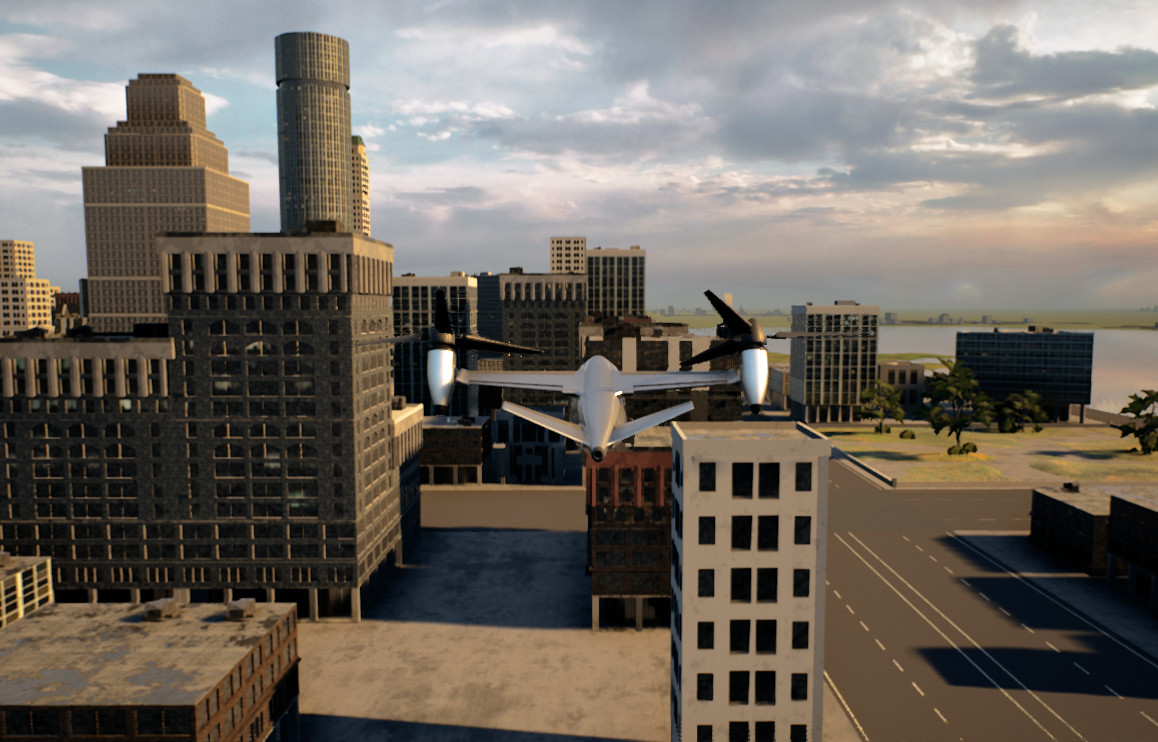
\includegraphics[height=250pt]{figures/vtol_example_geometric}
    \caption[Tiltrotor flying with geometric controller and PWM commands]{
        The tiltrotor vehicle flying in VTOL-AirSim with a geometric controller and control allocation module via PWM commands.}%
    \label{fig:vtol_example_geometric}
\end{figure}

\subsection{eVTOL Example --- Teleporting}\label{sec:vtol_teleport}
Inside the same \ci{geometric_control} directory of VTOLsim (see the previous section) is another script which does many of the same things as in the previous example, but instead of sending PWM commands to the motors, it directly sets the state of the aircraft. The script is named \ci{geometric_control_airsim_teleport.py}. It uses the same geometric controller and control allocation module, though it uses VTOLsim's dynamics simulation rather than VTOL-AirSim's. At each iteration of the main loop, VTOLsim computes the new state of the aircraft and sets the state of the aircraft in VTOL-AirSim through VTOL-AirSim's client command \ci{simSetVtolPose}. This method of using a graphics tool like AirSim for visualization of an external dynamics simulation is often referred to as \textit{teleporting}.

At the time of this writing, there are a few limitations to the teleport method. The first is that the tilt of the rotors cannot be animated. Although \ci{simSetVtolPose} has the parameter \ci{tilt_angles}, the implementation of setting the tilt angles of the rotors in this way is broken, and it produces bad results. We were not able to resolve the issue due to time constraints. For now, you should pass in values of \ci{np.nan} for the tilt angles (meaning the values won't be used), as is done in this script. The rotors will remain tilted at their \textit{nominal angle} --- set as 32.5\degree~for this aircraft --- throughout the flight. There is another parameter to the function, \ci{spin_props}, which if set to \ci{True} (the default value), should animate the spinning of the propellers, though with some minor visual artifacts.

The second limitation is that it requires using an environment compiled with a special zero gravity feature. With gravity, the aircraft can be successfully teleported to a pose in the world, but it begins falling between client calls of \ci{simSetVtolPose}. Without gravity, it stays at the commanded pose indefinitely. A version of the CityBlocks environment has been compiled specifically for this purpose, which we named \ci{CityBlocks_nogravity}. You need to download and use the latest version of the \ci{CityBlocks_nogravity} environment to run this teleport example.

in a terminal, start the \ci{CityBlocks_nogravity} environment. In another terminal session, navigate to the directory \ci{vtolsim/geometric_control}. Activate your virtual environment for VTOL-AirSim, then run:
\begin{minttcb}[title={Python Script for Teleporting}]{bash}
python3 geometric_control_airsim_teleport.py
\end{minttcb}

You should see the tiltrotor take off and travel from one rooftop to another, though without animation of the rotor tilts.

\subsection{eVTOL Example --- PX4 Integration}\label{sec:vtol_px4}
In this example, we will use the PX4 Autopilot to fly the tiltrotor. There are three items you need to run the example: the software \textit{QGroundControl}, the BYU-MAGICC fork of the PX4-Autopilot GitHub repository, and the right settings in your \ci{settings.json}.

Install QGroundControl by going to \url{https://docs.qgroundcontrol.com/master/en/getting_started/download_and_install.html}, then follow the instructions for Linux. Place the App Image file wherever you like; for example, in \ci{~/.local/bin}. Launch QGroundControl, then select your preferred units (metric is recommended).

Next, clone the \ci{byu-magicc/PX4-Autopilot} repository to somewhere on your machine, then switch to the \ci{v1.10.1-convergence} branch. We created this branch by making some additions to PX4 v1.10.1 in which we added the mixer for the E-flite Convergence airframe to the software-in-the-loop (SITL) configurations. The normal command you would run is \ci{make px4_sitl_default none_tiltrotor} to launch the PX4 firmware in SITL mode using the default tiltrotor mixer. We created the configuration \ci{none_convergence}, and this is the one you should use instead of \ci{none_tiltrotor}.

There are a number of extra settings that are needed for VTOL-AirSim to communicate with the PX4. The following settings should be in your \ci{settings.json} file:
\begin{minttcb}[title={Settings for VTOL-AirSim With PX4}]{json}
{
  "SettingsVersion": 1.2,
  "SimMode": "Vtol",
  "ClockSpeed": 1.00,
  "ViewMode": "SpringArmChase",
  "CameraDirector": {
      "FollowDistance": -20.0
  },
  "OriginGeopoint": {
    "Latitude": 40.246255,
    "Longitude": -111.647835,
    "Altitude": 1418
  },
  "Vehicles": {
    "uav0": {
      "VehicleType": "PX4Vtol",
      "Model": "TriTiltrotor",
      "UseSerial": false,
      "UseTcp": true,
      "TcpPort": 4560,
      "ControlPort": 14580,
      "Parameters": {
        "NAV_RCL_ACT": 0,
        "NAV_DLL_ACT": 0,
        "LPE_LAT": 40.246255,
        "LPE_LON": -111.647835,
        "COM_OBL_ACT": 1
      }
    }
  }
}
\end{minttcb}

The values for \ci{Latitude}, \ci{Longitude}, \ci{Altitude}, \ci{LPE_LAT}, and \ci{LPE_LON} were set for the Brigham Young University campus in Provo, Utah, USA. You may change these values to whichever location you are interested in simulating.

The \ci{ViewMode} and \ci{CameraDirector} settings are optional; however, we recommend using the \ci{SpringArmChase} mode in this example as it produces smoother visuals. You may find it useful to set this view mode in the other examples as well. Be aware that, in general, if you use \ci{SpringArmChase}, there is a bug in AirSim where the \ci{CameraDirector} is too close because of the 0.25 scale we set for the tiltrotor mesh to reduce its size. This makes it necessary to have a large value for \ci{FollowDistance}.

With the above settings, start running the CityBlocks environment. In another terminal, run the following command from within the directory containing the PX4-Autopilot repository:
\begin{minttcb}[title={}]{bash}
make px4_sitl_default none_convergence
\end{minttcb}

\begin{figure}[h]
    \centering
    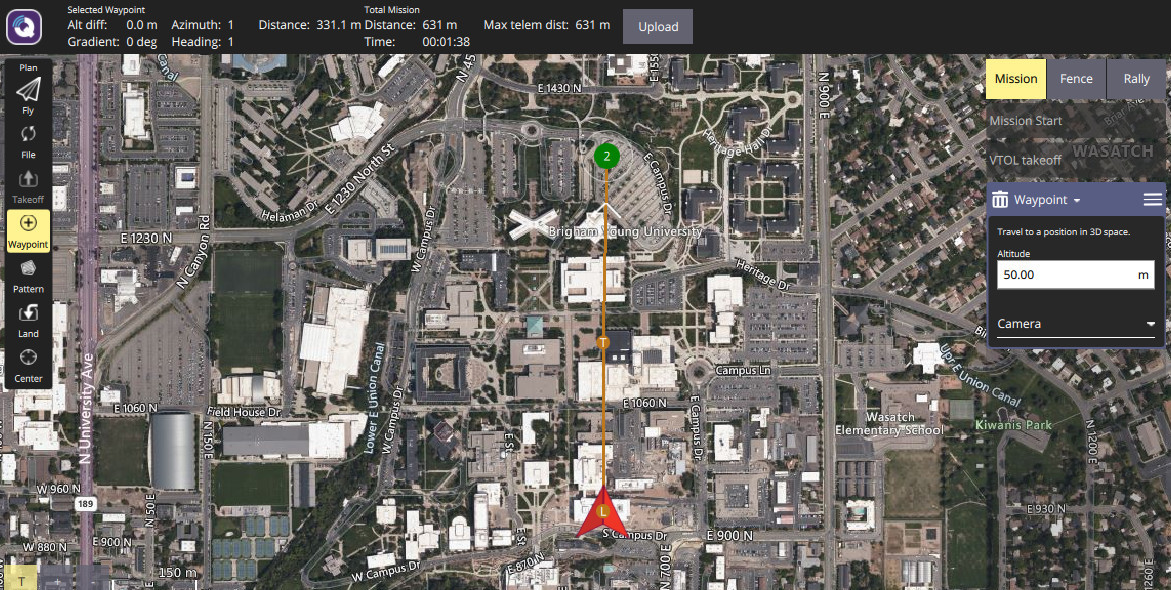
\includegraphics[width=\textwidth]{figures/qgroundcontrol_crop}
    \caption[QGroundControl showing mission plan]{
        QGroundControl screen after planning and uploading mission.}%
    \label{fig:qgroundcontrol}
\end{figure}

Next, launch QGroundControl. It should show the map centered around the detected GPS coordinate of the VTOL-AirSim vehicle (which are the values set for latitude and longitude in your settings). In the top-left of the map area, click \textbf{Plan}. Select \textbf{File} (if not already highlighted), then click \textbf{Blank}. Next, select \textbf{Takeoff}, and a green circle labeled \textbf{T} will appear (you may need to zoom out a bit to see it). You can click and drag the \textbf{T} to change the transition direction of the vehicle after takeoff, but we'll leave it there for this example. Click \textbf{Done} inside the \textbf{VTOL takeoff} box. Select \textbf{Waypoint}, then click somewhere to the north of the \textbf{T} circle. Finally, click \textbf{Upload Required} to upload the mission.  Your QGroundControl screen should look like Fig.~\ref{fig:qgroundcontrol}.

Now click \textbf{Fly}. There should be a slider button on the bottom that says \textit{Slide to confirm}. Slide the button to the right to send the mission to the tiltrotor in VTOL-AirSim. The tiltrotor should begin executing the mission (ignore any warning or error dialogs that pop up). It will first try to reach the target takeoff altitude, 50 m by default, then it will transition into fixed-wing mode in the direction that you set using the \textbf{T} circle. After that, it will head to the waypoint that you set, then after arriving, it will loiter about this waypoint --- i.e., orbit the waypoint indefinitely. It may actually hit a building while executing the mission; to avoid this, you can raise the altitude of the waypoints when planning the mission, or choose different waypoints.

\begin{figure}[h]
    \centering
    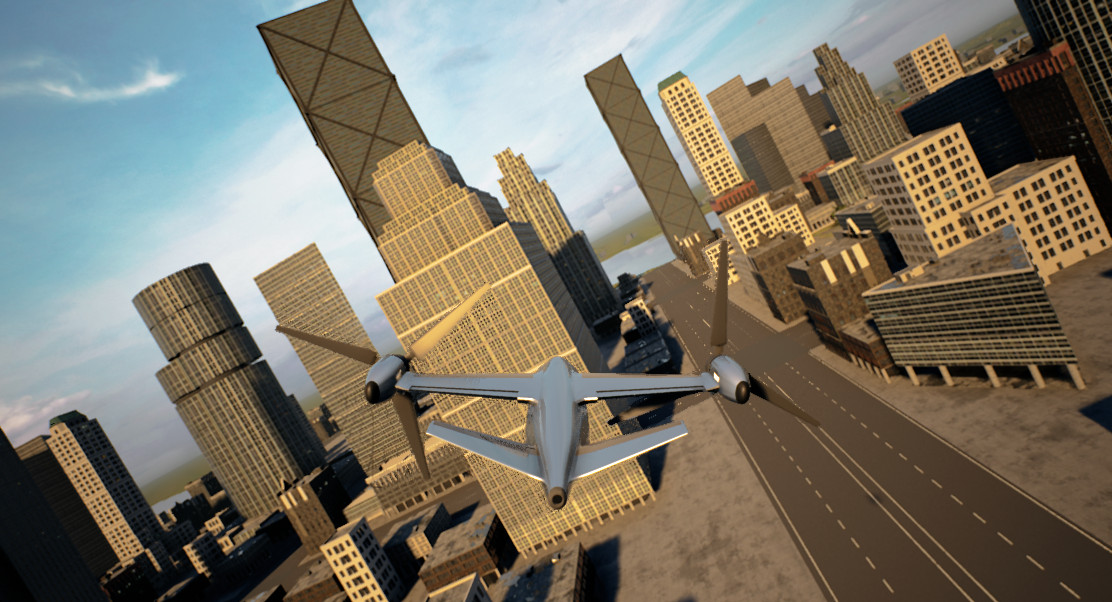
\includegraphics[width=\textwidth]{figures/vtol_example_px4}
    \caption[Tiltrotor flying with PX4 Autopilot]{
        The tiltrotor vehicle flying in VTOL-AirSim with the PX4 VTOL controller.}%
    \label{fig:vtol_example_px4}
\end{figure}